\documentclass[12pt]{article}
\usepackage[english]{babel}
\usepackage{natbib}
\usepackage{url}
\usepackage{listings}
\usepackage[utf8x]{inputenc}
\usepackage{amsmath}
\usepackage{graphicx}
\graphicspath{{images/}}
\usepackage{parskip}
\usepackage{fancyhdr}
\usepackage{vmargin}
\setmarginsrb{3 cm}{2.5 cm}{3 cm}{2.5 cm}{1 cm}{1.5 cm}{1 cm}{1.5 cm}
\lstset{language=C}
\title{Adding A System Call To The Linux Kernel}								% Title
\author{Hongru Huang}								% Author
\date{\today}											% Date

\makeatletter
\let\thetitle\@title
\let\theauthor\@author
\let\thedate\@date
\makeatother

\pagestyle{fancy}
\fancyhf{}
\rhead{\theauthor}
\lhead{\thetitle}
\cfoot{\thepage}

\begin{document}

%%%%%%%%%%%%%%%%%%%%%%%%%%%%%%%%%%%%%%%%%%%%%%%%%%%%%%%%%%%%%%%%%%%%%%%%%%%%%%%%%%%%%%%%%

\begin{titlepage}
	\centering
    \vspace*{0.5 cm}
    
\includegraphics[scale = 0.5]{sjtu_logo.jpg}\\[1.0 cm]	% University Logo
    \textsc{\LARGE Shanghai Jiao Tong University}\\[2.0 cm]	% University Name
	\textsc{\Large EI 338}\\[0.5 cm]				% Course Code
	\textsc{\large Computer System Engineering}\\[0.5 cm]				% Course Name
	\rule{\linewidth}{0.2 mm} \\[0.4 cm]
	{ \huge \bfseries \thetitle}\\
	\rule{\linewidth}{0.2 mm} \\[1.5 cm]
	
	\begin{minipage}{0.4\textwidth}
		\begin{flushleft} \large
			\emph{Author:}\\
			\theauthor
			\end{flushleft}
			\end{minipage}~
			\begin{minipage}{0.4\textwidth}
			\begin{flushright} \large
			\emph{Student Number:} \\
			515030910549									% Your Student Number
		\end{flushright}
	\end{minipage}\\[2 cm]
	
	{\large \thedate}\\[2 cm]
 
	\vfill
	
\end{titlepage}

%%%%%%%%%%%%%%%%%%%%%%%%%%%%%%%%%%%%%%%%%%%%%%%%%%%%%%%%%%%%%%%%%%%%%%%%%%%%%%%%%%%%%%%%%

\tableofcontents
\pagebreak

%%%%%%%%%%%%%%%%%%%%%%%%%%%%%%%%%%%%%%%%%%%%%%%%%%%%%%%%%%%%%%%%%%%%%%%%%%%%%%%%%%%%%%%%%

\section{Project Assignment}
In this project, you will study the system call interface provided by the Linux operating system and how user programs communicate with the operating system kernel via this interface. Your task is to incorporate a new system call into the kernel, thereby expanding the functionality of the operating system.
\section{Project Implementation}
This project is based on Linux Ubuntu 16.04.3 and the kernel version is 4.10.13. For other version of Ubuntu and kernel, this procedure is somewhat similar.
\subsection{Preparing}
Type the following commands to make sure the compiling process successfully:
\begin{itemize}
	\item \emph{sudo apt-get install gcc}
	\item \emph{sudo apt-get install libncurses5-dev}
	\item \emph{sudo apt-get update}
	\item \emph{sudo apt-get upgrade}
\end{itemize}
\subsection{Download the kernel}
At first I plan to complete this project just on the kernel provided by Ubuntu. It turns out that I can't do that because the kernel provided by Ubuntu is well-compiled and I can't find the source code, the \emph{syscall\_64.tbl} file and so on. The most important thing is that you can't compile the modified kernel without source code. Therefore the first step is to download a kernel with source code:
\begin{center}
\emph{
wget https://www.kernel.org/pub/linux/kernel/v4.x/linux-4.10.13.tar.gz}
\end{center}
After successfully downloading it, extract the kernel source code in \textbf{/usr/src/} directory using the following command:
\begin{center}
	\emph{sudo tar -xvf linux-4.10.13.tar.gz -C /usr/src/}
\end{center}
Then we can implement the project in directory \textbf{/usr/src/linux-4.10.13}.
\subsection{Define a new system call sys\_helloworld()}
Create a new directory \textbf{hello} in the kernel folder. And create a \textbf{helloworld.c} file in \textbf{hello} folder. This \textbf{.c} file is the source code of our new system call. You can check the source code in the project file. Note that We can't use the \textbf{printf} function here because this program runs in kernel mode and the \textbf{printf} function only works in user mode.

Create a \textbf{Makefile} in the \textbf{hello} folder add the following line:
\begin{center}
	\emph{obj-y := helloworld.o}
\end{center}
 A makefile is a special file, containing shell commands, that you create and name makefile (or Makefile depending upon the system). While in the directory containing this makefile, typing \emph{make} and the commands in the makefile will be executed. This line is to ensure that the \textbf{helloworld.o} will be compiled and included in the kernel source code.

\subsection{Modify the kernel}
\subsubsection{Add the hello directory to the kernel's Makefile}
Edit Makefile in the kernel folder. Find the line which says:
\begin{center}
core-y += kernel/ mm/ fs/ ipc/ security/ crypto/ block/
\end{center}
and change it as follows:
\begin{center}
	core-y += kernel/ mm/ fs/ ipc/ security/ crypto/ block/ hello/
\end{center}
We can find these files(\textbf{kernel}, \textbf{fs}, etc) in the kernel file. This is to tell the compiler that the source files of our new system call are in present in the \textbf{hello} directory.

\subsubsection{Add the new system call into the system call table}
My Ubuntu OS is 64bit. So firstly turn the directory \textbf{/arch/x86/entry/syscalls} and edit the file \textbf{syscall\_64.tbl}. Add the following line after $331_th$ system call
\begin{center}
	332\space\space\space\space64\space\space\space\space	helloworld\space\space\space\space\space\space\space\space		sys\_helloworld
\end{center}
Note that the blank is a tab not a space. $332$ is the number of the system call. This has to be noted down to make the system call in the userspace program.

\subsubsection{Add the new system call in the system call header file}
Turn to directory \textbf{/include/linux/} and edit file \textbf{syscalls.h}. Add the following line to the end of the file just before the \#endif  statement at the very bottom:
\begin{center}
	asmlinkage long sys\_hello(void);
\end{center}
This defines the prototype of the function of our system call. \textbf{asmlinkage} is a key word used to indicate that all parameters of the function would be available on the stack.

\subsection{Update the kernel}
\subsubsection{Compile the kernel}
To configure the kernel we need to use the following command:
\begin{center}
	\emph{sudo make menuconfig}
\end{center}
This command is used to configure the Linux kernel and it will pop up a window with lists of menus. In this project we just click \textbf{save} and \textbf{exit}.
\begin{center}
	\emph{sudo make oldconfig}
\end{center}
Then turn to the kernel file and type \emph{make} to compile the modified kernel. It will take us several hours of time.

\subsubsection{Install the kernel}
After successfully compiling the kernel, type the following command:
\begin{center}
	\emph{sudo make modules\_install install}
\end{center}
The command will install the Linux kernel 4.10.13 with our new system call\\ \textbf{sys\_helloworld}. After installation restart Ubuntu. If you type \emph{uname -r} after rebooting you will see the output kernel version is 4.10.13.

\subsection{Test the system call}
Recall that we use the \textbf{printk} function in the source file of our new system call, which will not display any information on the terminal but will display information in kernel's message. So we need another testing program to use the system call. You can check the test program in the project file.

Type \emph{gcc testprog.c} to compile the test program. We will get a \textbf{a.out} file. Then type \emph{./a.out} will display the information in the test program. Finally we can type \emph{dmesg} to scan the kernel's message. If all steps are done correctly we will see \textbf{"Hello World! Linux Kernel!"} at the end of the message just like this:
\begin{figure}
	\centering
	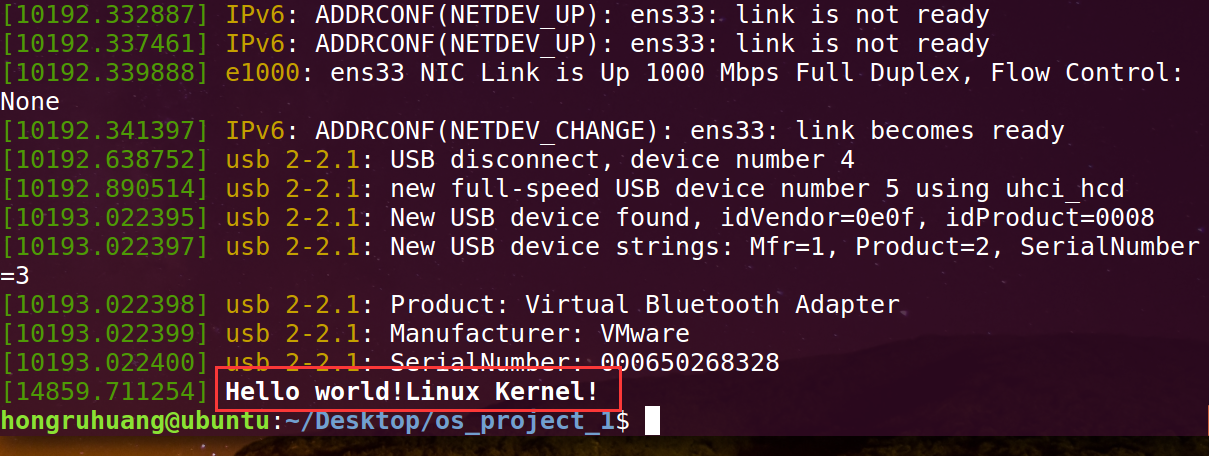
\includegraphics[scale=0.35]{result.png}
\end{figure}

\section{Conclusion}
This project gives me a deeper understanding about the kernel of Ubuntu Operating System. During this implementation procedure, I found many familiar files, like \textbf{stdio.h}, is visuable to us. This is very amazing because I think it is very secret before. And this makes me look at hello world program from another angle.

But there are many things I can't understand during this process, for example, the kernel configure window, which needs further study in this course.

\end{document}